\section{Overview and problem formulation}
\label{sec:overview}

We now present our method that takes as input an image sequence (or an image volume) containing a single object of interest and produces a pixel-wise segmentation of this object for all frames. In general, we assume that at most one object of interest is in the sequence and that part of the object is visible in each frame. For each frame in the sequence, we assume that a 2D location (\ie a pixel) within the object is provided by a user.
Hence, while we are interested in determining the entire object segmentation, the provided information only specifies local and compact regions of the object. These provided locations may be spatially disjoint and can refer to different or the same areas of the object. For this reason, our approach treats the task as a tracking problem where the image regions specified by the 2D locations must be jointly and coherently tracked so to recover the complete object segmentation. To do this, our approach hinges on two components. 

The first is a strategy to characterize the object of interest by using the provided image sequence and associated 2D locations. This is achieved by learning a classifier in a transductive fashion. In particular, we resort to bagging a set of decision trees. Instead of combining the aforementioned classifier with hand-crafted or learned features from large datasets, we learn features explicitly from the considered image sequence while using the 2D locations as a soft prior. This is achieved by training a U-Net architecture \cite{ronneberger2015} as an autoencoder in combination with a loss function that takes into account known object locations. By using the image features from this network, the classifier can then be used to assess the likelihood of image regions belonging to the object of interest.

The second component considers each specified 2D location as a potential target to track. To segment the object from these locations, we construct a graph over all compact image regions (\ie superpixels) in the image sequence.
The object segmentation is then inferred with a network flow optimization strategy whereby each of the provided 2D locations correspond to flow sources and we use the object likelihood to establish a series of costs between adjacent edges in our graph. We show that this graph can be optimized exactly and efficiently using a K-shortest path approach. To further improve the segmentation, we update our classifier using the previously found segmentation and repeat the K-shortest path optimization to produce an improved segmentation. This process is iterated until convergence of the final produced segmentation.

\comment{ 
\begin{figure}[!ht]
  \centering
\begin{tikzpicture}
  \centering
    \node[anchor=south west,inner sep=0] (image) at (0,0) {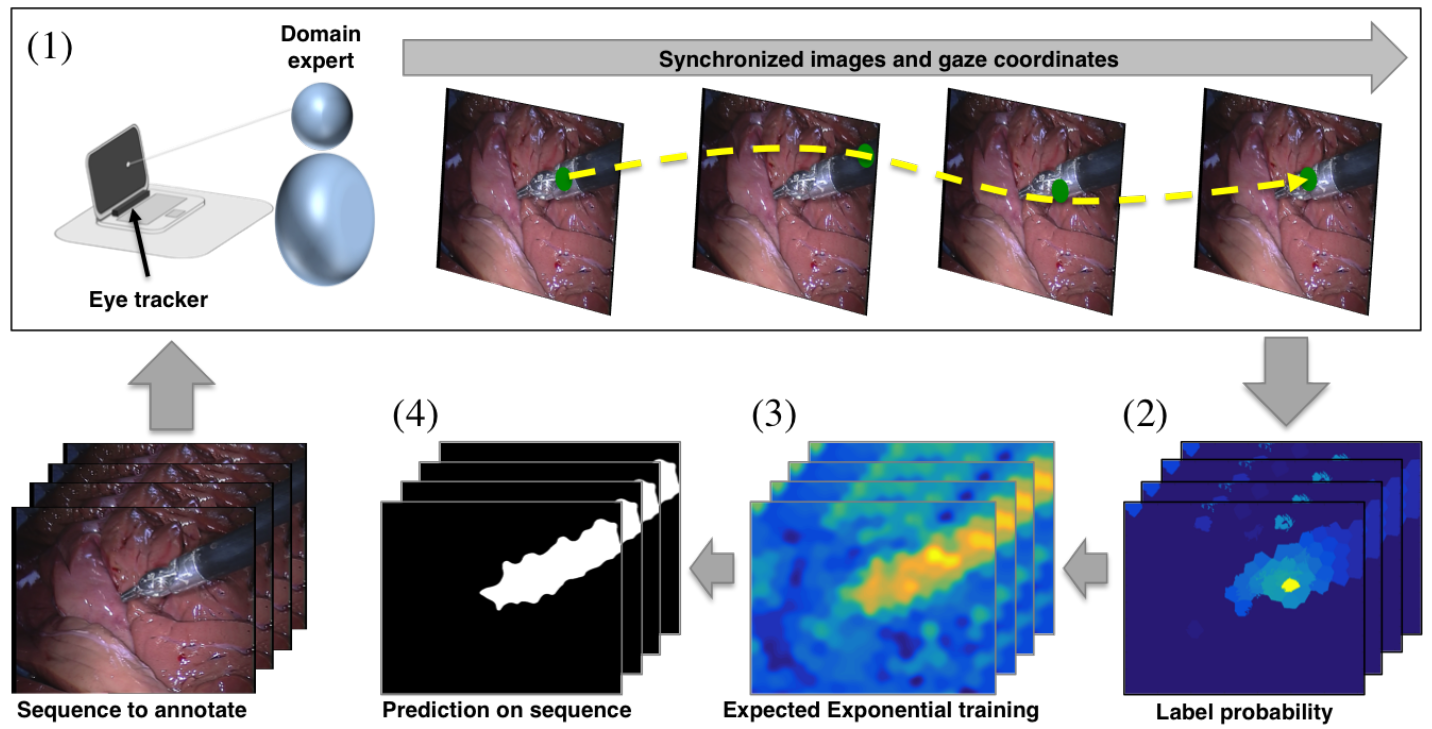
\includegraphics[width=0.7\textwidth]{pipeline}};
    \begin{scope}[x={(image.south east)},y={(image.north west)}]
        \node at (0.083,0.760)
    {Sec.~\ref{sec:features}};
        \node at (0.61,0.760)
    {Sec.~\ref{sec:optimization}};
    \end{scope}
\end{tikzpicture}
\caption{Full pipeline of our method.
  (Top) The dataset consists of a video/volumetric sequence and a set of 2D locations. (Middle) Our approach is divided in two main blocks: (Green frame) A feature learning phase where each pixels are assigned a feature vector. After a superpixel segmentation step, we assign to each superpixel a feature vector. (Red frame) A foreground model gives objectness likelihood to each superpixel. A MAP optimization problem then associates tracklets. Several iterations are performed and allow to re-train foreground and transition models. (Bottom) At the output, we obtain for each frame a binary segmentation of our object of interest.}
\label{fig:pipeline}
\end{figure}
}

By combining these two components, we show in our experiments that effective segmentations can be generated from extremely few 2D locations, without further prior assumptions on the image modality or the object of interest. 

We now briefly describe some notation that will be used throughout this paper and which are summarized in Table.~\ref{tab:notation}. Let the image sequence considered be denoted $\mathcal{I} = \{I_0,\ldots,I_T\}$ and let $\bm{g} = \{g_t\}_{t=0}^T$ with $g_t\in\mathbb{R}^2$ be a 2D pixel location in $I_t$. 
While we are ideally interested in a pixel-wise segmentation, we decompose each image as a set of superpixels so to reduce computational complexity. Given the volumetric nature of the problem considered, we opt to use 3D superpixels \cite{chang13} to group similar pixels over multiple frames. We thus let $I_t$ be described by the set of $N_t$ non-overlapping superpixels $S_t=\{s^n_t\}_{n=0}^{N_t}$ and define the set of all superpixels across all images as $\mathcal{S}=\{S_t\}_{t=0}^T$. In addition, we assign to each superpixel $s_t^n$ an appearance feature vector $a_t^n$ and define $\bm{a}=\{a_t^n | t=0,\ldots,T\quad n=0,\ldots,N_t\}$. We denote the set $\mathcal{S}^p = \{s^n_t | g_t \in s^n_t, t=0,\ldots,T,n=0,\ldots N_t \}$ as all superpixels observed and the rest as $\mathcal{S}^u = \mathcal{S} \setminus \mathcal{S}^p$.
\begin{table}[t!]
\begin{center}
\begin{tabular}{l l l}
\toprule
Symbol & Description\\
\toprule
$T$  & Number of frames\\
$I_t$  & Image at time $t$\\
$g_t$  & Coordinates of 2D location at time $t$\\
$N_t$  & Number of superpixels at time $t$\\
$s_{t}^n$  & Superpixel $n$ at time $t$ \\
$a_{t}^n$  & Feature vector of $s_t^n$\\
$u_{t}^n$  & Histogram of oriented optical flow of $s_t^n$\\
$Y_{t}^n$  & Binary random variable that models objectness of $s_t^n$\\
$\rho_{t}^n$  & Probability of $s_t^n$ being object given the object model\\
$\mathcal{T}_{t}^n$  & Tracklet starting at time $t$ and superpixel $n$\\
$r_{t}^n$  & Centroid of $s_t^n$\\
$e_{t}^n$, $f_{t}^n$, $C_{t}^n$ & Edge, flow and cost for passing through $\mathcal{T}_t^n$\\
$e_t^{n,m}$, $f_t^{n,m}$, $C_t^{n,m}$  & Edge, flow and cost for linking $\mathcal{T}_t^n$ and $\mathcal{T}_{t+1}^m$\\
$e_t^{\mathcal{E},n}$, $f_t^{\mathcal{E},n}$, $C_t^{\mathcal{E},n}$  & Edge, flow, and cost for entering the network from $\mathcal{T}_t^n$\\
$\tau_{\rho}$  & Threshold applied on edges $e_t^n$ according to $\rho_t^n$\\
$\tau_{u}$  & Threshold applied on edges $e_t^{n,m}$ according to $u_t^n$\\
$\tau_{trans}$  & Threshold on edges $e_t^{i,j}$ and $e_t^{g,n}$ according to $u_t^n$\\
$R$  & Radius around 2D location (entrance), and tracklet transitions \\
$Z_{t}$  & Objectness prior at time $t$\\
$\sigma_{g}$  & Standard-deviation of objectness prior for feature extraction\\
\bottomrule
\end{tabular}
\end{center}
\caption{Notation summary}
\label{tab:notation}
\end{table}


%-----------------------------------------------------%
%-----------------------------------------------------%
%-----------------------------------------------------%

\section{Transductive foreground model}
To build a model of the object appearance, we take a transductive learning approach. Here we follow a P-U learning scheme in which only a few positive samples are given along with a larger set of unknown samples. In practice for an image, we expect one superpixel to be annotated compared to hundreds of unobserved ones. While using Neural Networks would be effective for supervised binary segmentation problems, it is unclear what loss function one should minimize in a P-U regime. Instead, we propose to train a simple bagging classifier with novel features that are both image and object specific, and allow coarse superpixel regions to be characterized. 

\subsection{Probabilistic estimation by bagging}
\label{sec:foreground_model}
To build a prediction model, we train $M$ binary decision trees by using different data subsets. Each tree takes as input the feature vector $a_t^n \in \mathbb{R}^D$ characterizing the superpixel $s_t^n$ and estimates $Y_t^n \in \{0,1\}$, where $Y_t^n = 1$ if it belongs to the object and $0$ otherwise. For each tree, the entire positive set $\mathcal{S}^p$ is used for training, in addition to $|\mathcal{S}^p|$ randomly selected samples with replacement from the unlabeled set $\mathcal{S}^u$. The latter are treated as negative samples. The trees are then trained using the Gini impurity loss function \cite{menze09}, with $\sqrt{D}$ randomly selected features considered at each node of a tree. Then for a given superpixel $s_t^n$, the probability that it is part of the object, $\rho_{t}^n = P(Y_t^n = 1 | a_{t}^n )$ can be computed by averaging the predictions over all $M$ trees.

\subsection{Image-object specific features}\label{sec:features}
In general, there are many different features that could be used in the above classifier. In this context however, we wish to use features that are effective for segmenting a specific object in a given image modality. That is, we are interested in learning features that are both image-object specific (IOS), but do not need to generalize to other unseen data. 

To this end, we learn features by making use of an autoencoder neural network. As illustrated in Fig.~\ref{fig:unet}, we let the network take as input an image from a sequence and is tasked to predict the same image as output. In our network, we use three stacked convolutional layers with $3 \times 3$ filter with strides of $1$ per level in an encoding and decoding path. We also perform batch normalization with ReLU activations after each convolutional layer. The last layer is a convolutional layer with filter size $1 \times 1$ and a sigmoid activation. In practice, as our network has $4$ levels, where we first downscale the images to the nearest width and height divisible by $16$.

While such an autoencoder can be trained by minimizing the $L^2$-norm \cite{vincent08}, we are interested in forcing the network to have strong performances on regions of the object of interest rather than on potentially irrelevant parts of the image. As such, we propose to impose an ``objectness prior", which we add to our loss function in the form of a soft constraint. Specifically, we define ${Z}_t \sim \mathcal{N}(g_t, \sigma_g^2\bm{1})$ to be a 2D weighted map of the same size as $I_t$. The mean of this image is centered on the location $g_t$ and has symmetric variance $\sigma_g^2$. We then integrate this map in our loss as
\begin{equation}
\mathcal{L} = \sum_{{I}_t \in \mathcal{I}} \sum_{k,l} {Z}_t(k,l) \| I_t(k,l) - {\hat{I}}_t(k,l)\|^2,
\label{eq:loss_features}
\end{equation}
\noindent
where $\hat{I}_t$ is the output of the network, $k$ and $l$ are pixel indices in a $W \cdot H$ sized image $I_t$. In effect, this loss penalizes incorrect reconstructions  more heavily on the regions that are known to be part of the object.

After training, a forward pass is performed on an image and features of dimension $512$ are extracted at the output of the deepest layer. These features correspond to a downscaled version of the input image which are then upscaled to the original image size using bicubic interpolation. The feature vector associated to a superpixel $s_t^n$ is then taken to be the mean over all pixels contained within it,
\begin{equation}
\begin{split}
  a_t^n = \frac{1}{|s_t^n|} \sum_{(k,l) \in s_t^n}h_t(k,l),
\end{split}
\label{eq:app_vector}
\end{equation}
\noindent
where $h_t(k,l) \in \mathbb{R}^{512}$ is the feature vector extracted at pixel $(k,l)$. As we will show in our experiments, this strategy generally improves the overall performance of our method.

\begin{figure}[t]
\centering
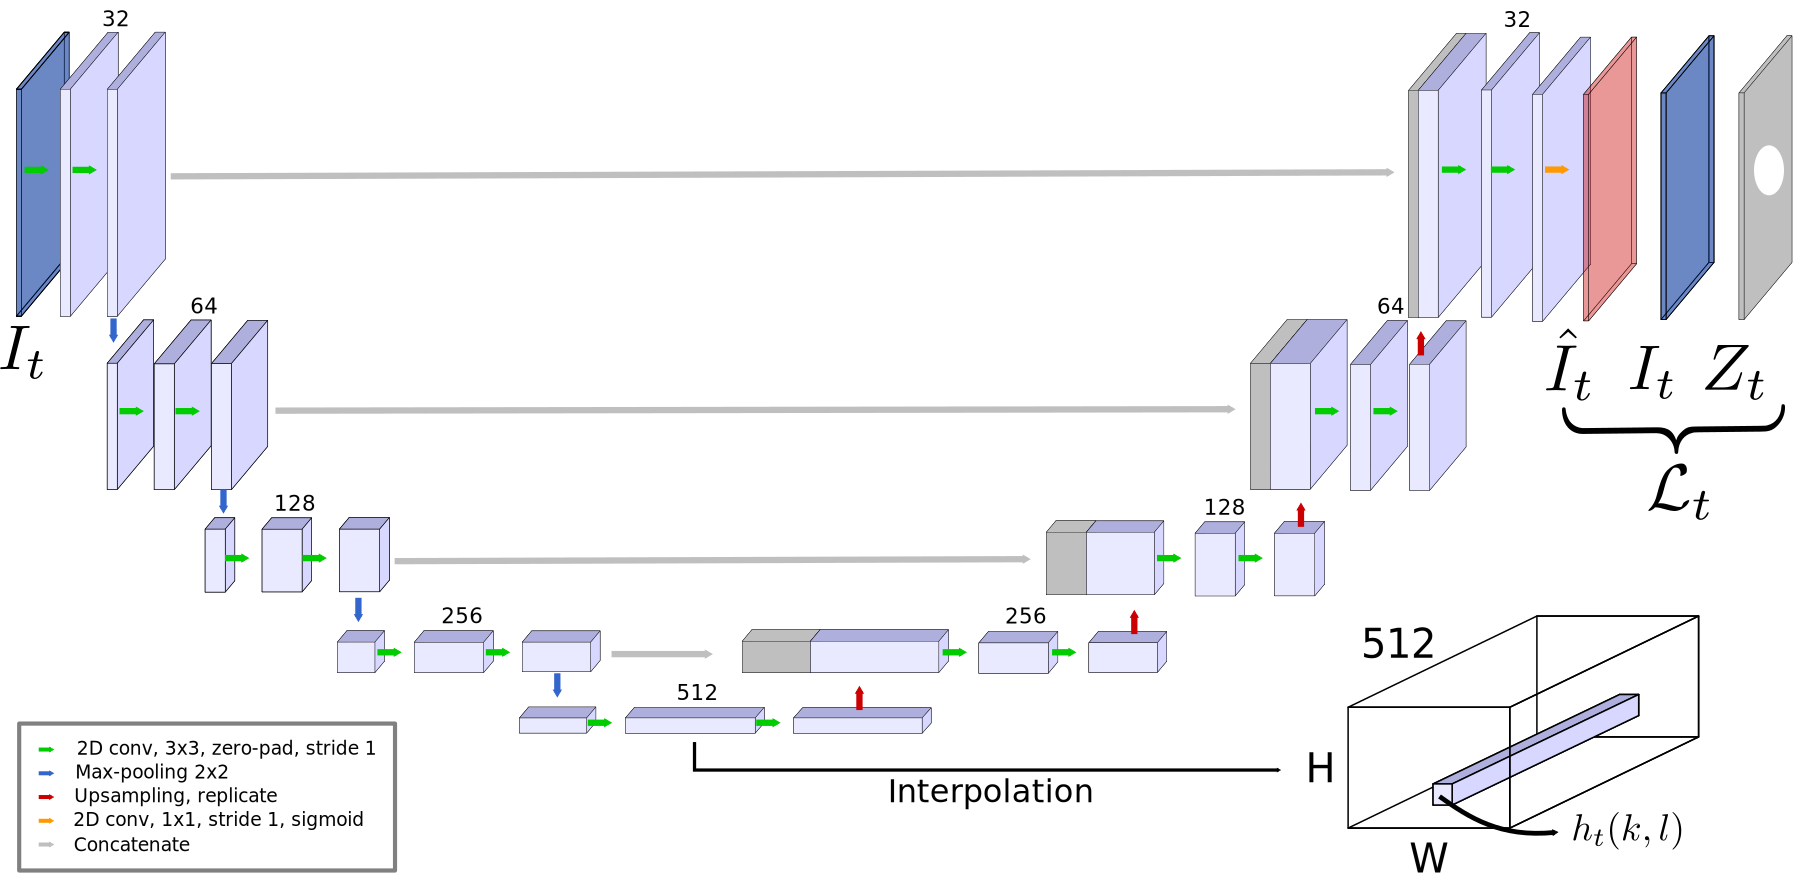
\includegraphics[width=1\textwidth]{fig2}
\caption{Image-object specific features. The network is tasked to reconstruct the input image $I_t$ (dark blue). By means of a loss function $\mathcal{L}_t$, the reconstructed image, $\hat{I}_t$ (red), is strongly penalized at 2D locations provided by means of the soft prior, $Z_t$. At test time, the features $h_t(k,l)$ are extracted by interpolating the bottom layer to the original input size.
}
\label{fig:unet}
\end{figure}
%------------------------------------------------------------------%
%------------------------------------------------------------------%
%------------------------------------------------------------------%

\section{Segmentation by tracking} \label{sec:optimization}
Given the above local object model, we wish to provide a global strategy to infer an accurate segmentation of the object across all frames. As we make no assumption on the object of interest (\eg shape, color, motion, etc.), we \blue{hypothesise} that by tracking these local regions over the entire data volume, that a complete segmentation of the object can be coherently inferred. That is, we consider each region specified by a provided 2D location to be an individual target, that could potentially depict different parts of the same object. In what follows, we show how these different regions can be tracked optimally so as to provide the complete object segmentation.

\subsection{MAP Formulation}\label{sec:MAP}
To track the 2D locations as function of the object, we define $\bm{Y} = \{Y_t^n|\forall(t,n)\}$ as the set of all $Y$ labels.
As defined in Sec.~\ref{sec:overview}, $\bm{g}, \bm{a}$ are the grouping variables of the provided 2D locations and the extracted superpixel features, respectively.
We then define our segmentation problem as a Maximum a posteriori (MAP) optimization,
    \begin{equation}
    \begin{split}
    y^* = \arg \max_{y \in \mathcal{Y}} P(\bm{Y}=\bm{y}|\bm{a}, \bm{g}),
    \end{split}
    \label{eq:map}
    \end{equation}
\noindent
where $y^*$ is the sought out binary labels for all frames. Assuming that $Y_t^n$ is conditionally independent given the observed variables $\bm{a}$, we rewrite Eq.~\eqref{eq:map} as,
    \begin{equation}
    \begin{split}
    y^* = \arg \max_{y \in \mathcal{Y}} \prod_{\substack{m,n,t}} P(Y_t^{n}|\bm{a},\bm{g}) P(Y_t^{n}|a_{t-1}^{m})P(Y_t^{n}|a_t,g_t).
    \end{split}
    \label{eq:map2}
    \end{equation}
\noindent
In particular, the three terms of the decomposition of Eq.~\eqref{eq:map2} correspond to different aspects of the object appearance models. Concretely,
\begin{itemize}
\item[-]  {$P(Y_t^{n}|\bm{a},\bm{g})$} is modeled using our classifier (Sec.~\ref{sec:foreground_model}) and behaves as an object appearance model. 
\item[-] {$P(Y_t^{n}|a_{t-1}^{m})$} models the similarity between two superpixels in successive frames, so to describe how frame-to-frame probabilities propagate. 
\item[-] {$P(Y_t^{n}|a_t,g_t)$} models the likelihood that a given superpixel $s_t^n$ is visually similar to the one selected by the 2D location $g_t$. In practice, in the case where the object of interest is large and visually homogeneous, this term allows to initiate several tracks for a single given 2D annotation.
\end{itemize}

While optimizing Eq.~\eqref{eq:map2} appears complex, we show in the following section that it can be performed efficiently by means of an integer program formulation and a K-Shortest Path optimization. %$P(Y_t^{n}|a_{t-1}^{m})$ and  $P(Y_t^{n}|\bm{a},g_t)$ models are further described in Sec.~\ref{sec:costs}. 

\subsection{Flow network formulation}
\label{sec:solving}
Thanks to its inherent structure, our MAP problem can be mapped into a cost-flow problem and can be solved efficiently. Specifically, we wish to determine where flow emitted from a source node must traverse a graph in order to minimize the traversal cost to a sink node \cite{zhang08}. For that matter, we associate to each superpixel $s_t^n$ a tracklet $\mathcal{T}_t^n$ (\ie an edge that represents the entrance and exit of a superpixel) and define $r_t^n\in \mathbb{R}^2$ as the central pixel of superpixel $s_t^n$. Fig.~\ref{fig:mcf} shows a graphical representation of our flow network formulation.

%\subsubsection{Integer Program}
%\label{sec:int_prog}
As a first step, the MAP problem of Eq.~\eqref{eq:map2} is transformed into an Integer Program (IP) \cite{schrijver98}. To simplify notations, let $\alpha_t^{m,n} \coloneqq P(Y_t^n=1|a_{t-1}^m)$, $\beta_t^n \coloneqq P(Y_t^n=1|a_t,g_t)$, and $\rho_t^n \coloneqq P(Y_t^n=1|\bm{a},\bm{g})$. We also introduce a sink node $\mathcal{X}$, and set of source nodes $\mathcal{E}_t$ such that each pushes flow onto the corresponding frame $I_t$.
Additionally, we introduce the variables $f_t^n$, $f_t^{m,n}$, $f_t^{\mathcal{E},n}$, and $f^{n,\mathcal{X}}$ to denote tracklet, transition, entrance and exit flows, respectively. The corresponding IP is thus given by,
  \begin{subequations}
  \label{eq:int_prog}
  \begin{align}
  \intertext{Maximize}
  &\sum_{t,n} \log{\frac{\rho_t^n}{1-\rho_t^n}}f_t^n + \sum_{t,m} \log{\frac{\alpha_t^{m,n}}{1-\alpha_t^{m,n}}}\sum_{t,n}f_t^{m,n} + \sum_{t,n} \log{\frac{\beta_t^n}{1-\beta_t^n}}f_t^{\mathcal{E}_t,n},\label{eq:loglikelihood}\\
  \intertext{subject to,}
  &\sum\limits_{n}f_t^{m,n} \leq 1, \qquad \forall t,m,n \label{eq:cap1_trans}\\
  &\sum_m f_t^{m,n} - \sum_p f_{t-1}^{p,m} \leq 0, \qquad \forall t,m,n,p \label{eq:conserv1}\\
  &\sum_{m,t} f_t^{\mathcal{E}_t,m} - \sum_p f^{p,\mathcal{X}} \leq 0, \qquad \forall t,m\label{eq:conserv2}
  \end{align}
  \end{subequations}
\noindent
where the above objective function, Eq.~\eqref{eq:loglikelihood}, corresponds to the log-likelihood of Eq.~\eqref{eq:map2} and where each flow variable associated to a cost term corresponds to a Bernoulli variable. The constraint defined by Eq.~\eqref{eq:cap1_trans} imposes a maximum flow capacitance of value one, thereby expressing the assumption that a superpixel can only contain a single target. Eq.~\eqref{eq:conserv1} imposes flow conservation, \ie at each node the input flow must be equal to the output flow (except for the source and sink nodes). Last, Eq.~\eqref{eq:conserv2} imposes that the sum of flow emitted by the source node $\mathcal{E}$ must reach the sink node $\mathcal{X}$. By design, the solution of this IP gives $Y_t^n=1$ if $f_t^n$ is equal to the edge capacity and 0 otherwise.
\begin{figure}[t]
\centering
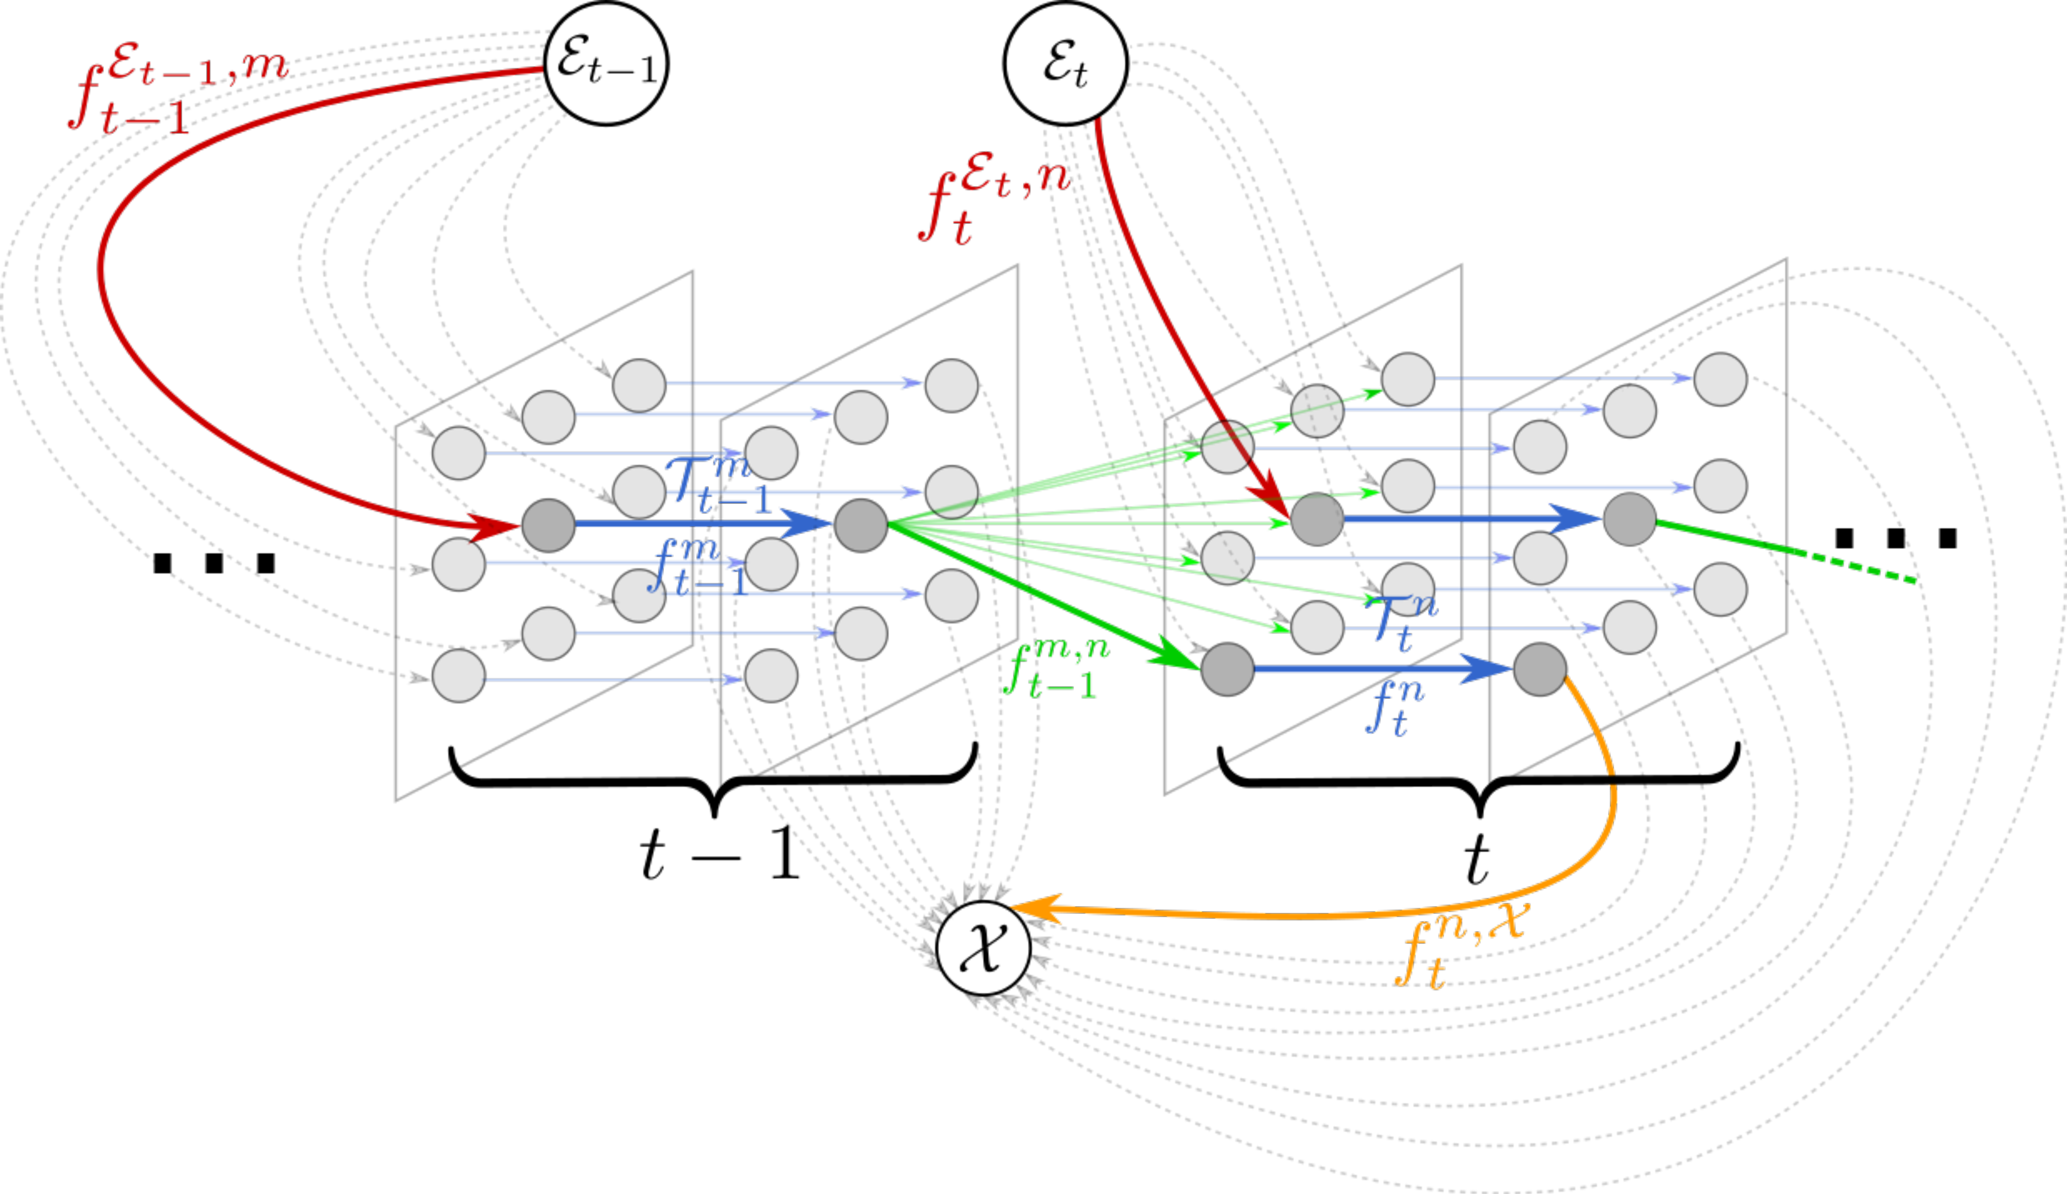
\includegraphics[width=1\textwidth]{fig3}
\caption{Max-Flow graph (forward case). At each time frame $t$, a ``pseudo'' source node $\mathcal{E}_t$ is connected via an edge with flow $f_{t}^{\mathcal{E},n}$ (red) to tracklet $\mathcal{T}_t^n$. Each tracklet incurs a flow $f_t^n$ (blue) to pass through a superpixel $s_t^n$. Tracklets in frame $t$ are connected to tracklets in the next frame and allow for flows $f_{t}^{m,n}$ (green). The flow $f_{t}^{n,\mathcal{X}}$ can leave any tracklet in the network (orange).}
\label{fig:mcf}
\end{figure}

To further specify constraints for our given application, we now outline three additional edge-pruning measures. While these could be added directly in Eq.~\eqref{eq:loglikelihood}, we opt to describe them here instead.
\begin{itemize}
\item[-] {\bf Entrance edge pruning:} The provided 2D locations allow for a strong prior on the location of the object. Intuitively, we wish to force flow where the 2D locations are known (\ie $g_t$). We therefore connect $\mathcal{E}_t$ to all $\mathcal{T}_t^n$ such that the centroid of the corresponding superpixel, $r_t^n$, is included in a neighborhood centered at $g_t$ with radius $R$ (see Fig.~\ref{fig:temporal_merge}(left)). % $\mathcal{N}(g_t,R)$, a circle centered at $g_t$ with radius $R$. 
The parameter $R$ therefore control the quantity of flow that can be pushed from a given source node into its corresponding image. Edges that do not fulfil this condition are pruned.

\item[-] {\bf Transition edge pruning:} For edges that link tracklets, we use location and motion constraints to remove edges. For locations, we prune edges where $r_{t}^n$ is outside of a neighborhood centered on $r_{t-1}^m$ of radius $R$. Similarly, we estimate  superpixel motion by means of a histogram of oriented optical flow \cite{chaudhry09}. Defining this motion by $u_t^n\in \mathbb{R}^l$, we prune edges such that $S_m(u_{t-1}^m,u_t^n) < \tau_u$, where $S_m(\cdot,\cdot)$ is the histogram intersection similarity.

\item[-] {\bf Tracklet edge pruning:} We let the probabilistic estimation described in Sec.~\ref{sec:foreground_model} be related to the cost of pushing flow through tracklets. Depending on the sequence, this estimate can lead to false positives (\ie give a high probability value on the background). To circumvent this phenomenon, we prune tracklet edges whose probability are below a threshold, $\rho_t^n < \tau_\rho$.
\end{itemize}

Note that given this IP formulation, the number of pseudo source nodes $\mathcal{E}_t$ does not change the optimization problem of Eq.~\eqref{eq:loglikelihood}. This implies that whether multiple 2D locations or none were be specified on each frame $t$, the IP would remain unchanged. Naturally, omitted source nodes on frames would reduce the quality of the solution as less information would be available to the foreground model (sec.~\ref{sec:foreground_model}). However, as we will show in our experiments, our global optimization recovers paths that span several frames and limits the impact of such cases. Similarly, the pruning of edges does not affect the solution of Eq.~\eqref{eq:loglikelihood} given that these would have infinite cost were they to be explicitly kept, and thus never allow flow to pass through them. 

\subsection{K-shortest path optimization}
As with all IP optimization problems, Eq.~\eqref{eq:int_prog} is NP-hard \cite{papadimitriou81}. However, as noted in~\cite{berclaz11}, our problem can be relaxed to a Linear Program thanks to the total unimodularity of the constraints matrix. The latter condition guarantees that the solution will converge to an integer solution, making off-the-shelf optimizers suitable (\eg Simplex \cite{klee70}, Interior point \cite{kojima89}). However, we use a more efficient alternative -- the K-shortest paths algorithm (KSP) applied to the case where all edges have unit capacitance.
In contrast with generic LP solvers, KSP explicitly leverages the connectivity of nodes in the graph.
While~\cite{berclaz11} used a node-disjoint optimization to restrict nodes from receiving flow from different sources, our tracklet costs, $C_t^n$, allow a simpler edge-disjoint K-shortest paths algorithm by minimizing the negative of Eq.~\eqref{eq:loglikelihood}.
We provide further details on our implementation in Appendix A.

Last, to take into account information from previous and future frames, we compute both a forward and backward graph so to track superpixels forward and backward in time. This gives rise to two independent MAP problems to solve: one in each time direction. While we only present the forward case here, the backward case can easily be derived. The final labeling of a sequence is then given by the union of the two solution sets.

\subsection{Model costs}\label{sec:costs}
In what follows, we describe in detail how edge costs associated to Eq.~\eqref{eq:loglikelihood} are computed.

\begin{itemize}
\item[-]{{\bf Tracklet costs:}} As indicated in Sec.~\ref{sec:solving}, $\rho_{t}^n$ is the probability that the superpixel $s_t^n$ is part of the object according to the classifier. The cost of the corresponding flow $f_t^n$ is thus given by
\begin{equation}
C_{t}^n = -\log \frac{\rho_t^n}{1-\rho_t^n}
\label{eq:in_frame_cost}
\end{equation}
\noindent
and is illustrated with blue edges in Fig.~\ref{fig:mcf}. 

\item[-]{{\bf Transition costs:}} We model $\alpha_t^{m,n}$, the likelihood that superpixels $s_t^n$ and $s_{t+1}^m$ correspond to the same region in the sequence. In our flow-network, this corresponds to the cost of transiting from tracklet $\mathcal{T}_t^n$ to $\mathcal{T}_{t+1}^m$ (green edges in Fig.~\ref{fig:mcf}). 

While defining costs based on image features for such transitions is complex when the object size and background is unknown, we propose to learn and use an appropriate representation instead. In particular, we use Local Fisher Discriminant Analysis (LFDA), a supervised metric learning method \cite{sugiyama06}, to measure the appearance similarity between two superpixels. In addition to Fisher Discriminant Analysis (FDA) \cite{welling05}, which maximizes between-class scatter while minimizing within-class scatter, LFDA considers multi-modal classes, thereby preserving the local structure of data. In practice, we set the two LFDA parameters empirically: The $k$ nearest-neighbour data points used to compute an affinity matrix, and $Q$, the dimension of the output space. We select as positive samples the $a_t^n$ with associated probability $\rho_t^n$ larger than a threshold $\tau_{trans}$. As negatives, we randomly select an equal amount of samples below that threshold. Letting $V$ be the LFDA projection matrix, we set
\begin{equation}
  \alpha_{t}^{m,n} = \exp \left( {-|| V(a_t^n - a_{t+1}^{m})||^2_2} \right),
\label{eq:alpha}
\end{equation}
\noindent
and the flow cost $f_t^{m,n}$ is then given by
\begin{equation}
C_{t}^{m,n} = -\log\frac{\alpha_{t}^{m,n}}{1-\alpha_{t}^{m,n}}.
\end{equation}

\item[-]{{\bf Entrance-Exit costs:}}
The source nodes $\mathcal{E}_t$ allow flow to be pushed through the network. Intuitively, at a given frame, we want to push flow starting from superpixels that are similar to the region given by$g_t$. Letting $\beta_t^n = P(Y_t^{n}|a_t,{g}_{t})$ denote the probability of entering the network from $\mathcal{T}_t^n$, we compute,
\begin{equation}
  \beta_{t}^n = \exp \left( -|| V(a_t^n - a_t)||^2_2 \right)
\label{eq:beta}
\end{equation}
where $V$ is the previously computed LFDA projection matrix, $a_t$ corresponds to the feature vector of the superpixel selected by $g_t$, whereas $a_t^n$ corresponds to the superpixel feature vector in question. The flow cost associated $f_{t}^{\mathcal{E}_t,n}$ (red edges in Fig.~\ref{fig:mcf}) is then taken as $C_{t}^{\mathcal{E}_t,n} = -\log(\beta_{t}^n / (1-\beta_{t}^n))$. In addition, since we do not model the likelihood of terminating a path, we set the cost of exiting to the sink node $C_{t}^{n,\mathcal{X}}$ to be 0 for all tracklets.
\end{itemize}

\begin{figure}[t]
\centering
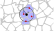
\includegraphics[width=0.49\textwidth]{fig4a}
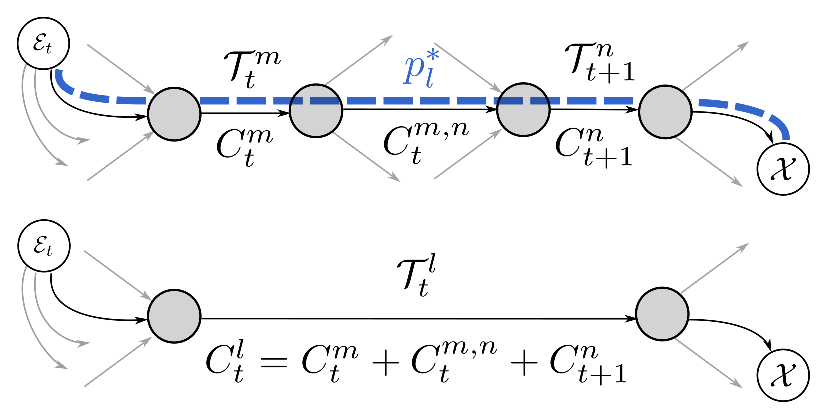
\includegraphics[width=0.49\textwidth]{fig4b}
\caption{(left) Flow entrance. Superpixel boundaries are drawn in grey. All superpixels whose centroids (red circles) are contained in a circle of radius $R$ will accept entrance flow. (Right) Example of a temporal merge. Top: Path $p_l^*$ (in blue) crosses tracklets $\mathcal{T}_t^n$ and $\mathcal{T}_{t+1}^{m}$. Bottom: At the next iteration, the corresponding tracklets merge into a single tracklet $\mathcal{T}_t^{l}$ with cost $C_t^n + C_{t}^{m,n} + C_{t+1}^{m}$.}
\label{fig:temporal_merge}
\end{figure}

%------------------------------------------------------------------%
%------------------------------------------------------------------%
%------------------------------------------------------------------%

\subsection{Iterative tracking}
\label{sec:iterative_ksp}
Given that our object model described in Sec.~\ref{sec:foreground_model}, is trained on very few positive samples, solving Eq.~\eqref{eq:loglikelihood} can lead to a number of missed positive superpixels. To circumvent this limitation, we propose to augment the positive set $\mathcal{S}_p$ in an iterative way, by adding new positive samples recovered from our produced KSP estimation. That is, after initially inferring the object segmentation, new object superpixels are considered as positive samples in order to re-train the classifer and recompute the graph costs. 

To do this, the costs $C_t^n$, $C_{t}^{m,n}$ and $C_{t}^{\mathcal{E},n}$ are updated after each KSP optimization. More specifically, we define $\mathcal{P^*} = \{ p_0^*,...,p_{K-1}^*\}$ to be the set of solution paths given by the KSP optimization, with $p_l^*$ being the set of tracklets in path $l$. We make the assumption that at the next iteration, the solver would most likely extend found paths given by the previous result. We can then merge tracklets belonging to the same path (\ie concatenate them temporally to form a new tracklet). This brings the practical advantage of reducing the complexity of our problem as the number of edges decreases at each iteration. 

In this case, we set the edge cost following the merge to be
\begin{equation}
\begin{split}
  C_l := \sum_{n,t}C_t^n + \sum_{m,n,t}C_{t}^{m,n}
\end{split}
\label{eq:cost_transform}
\end{equation}
\noindent
with tuples $(n,t)$ and $(m,n,t)$ corresponding to edges occupied by path $p_l^*$. The algorithm then terminates when no new tracklets are added to the set $\mathcal{P}$. Fig.~\ref{fig:temporal_merge}(right) illustrates this temporal merging step while the pseudo code of our iterative solver, which we denote \KSP, is shown in Alg.~\ref{alg:iter_ksp}. Fig.~\ref{fig:example_iter_ksp} shows example frames of how different samples are sequentially added to the positive set, allowing for better classification and KSP solutions.

\begin{figure}[t]
\centering
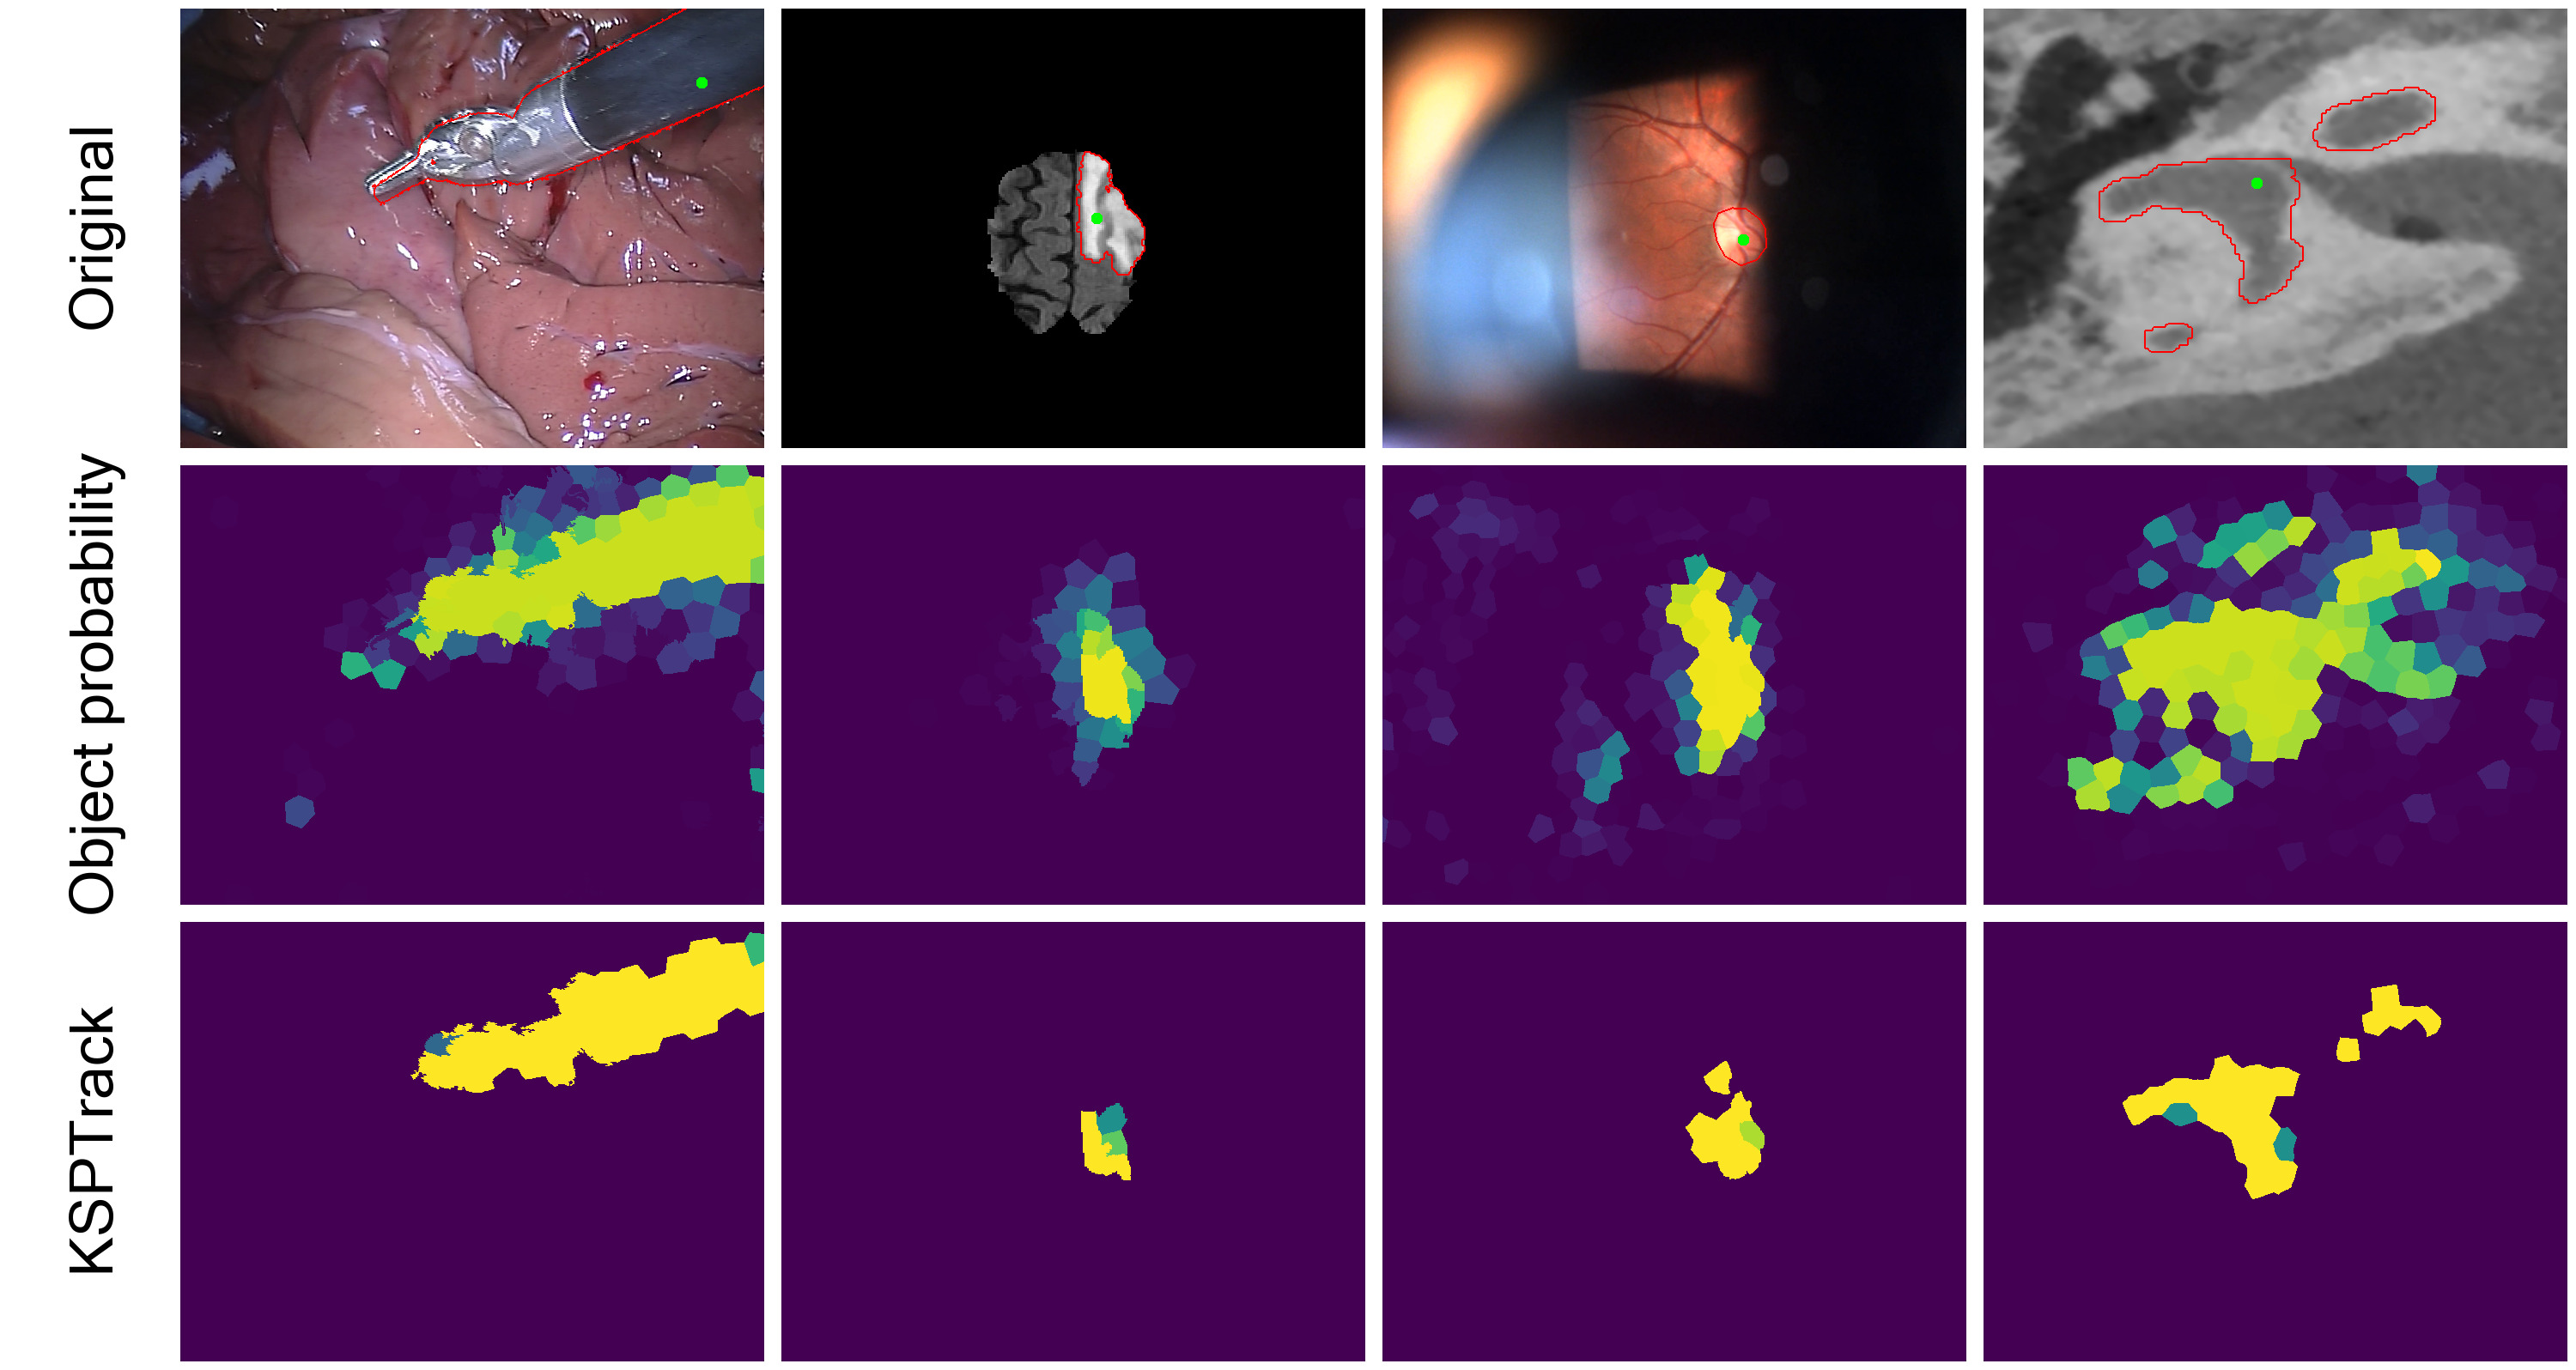
\includegraphics[width=0.99\textwidth]{fig5.jpg}
\caption{(Top row): Original images from different datasets. Ground truth contour of the structure of interest is depicted in red and the supervised 2D locations are shown in green.
(Middle row): $\rho_{t}^n$, probability estimates of the object given by our classifier after the final iteration of our approach.
(Bottom row): Pixel-wise sum of binary segmentations after each iteration of the KSP optimization. Total number of iterations from left to right are: $3$, $4$, $3$, $2$.}
\label{fig:example_iter_ksp}
\end{figure}

\begin{algorithm}[t]
\SetKwInOut{Input}{Input}
\SetKwInOut{Output}{Output}
\DontPrintSemicolon
\Input{$\mathcal{S}_p$: Initial set of positive superpixels, $\mathcal{S}_u$: Initial set of unlabeled superpixels, $\mathcal{S}$: set of superpixels (with associated variables $\bm{a}$, $\bm{u}$, and $\bm{r}$), $\mathcal{G}$: 2D locations}
\Output{$\mathcal{P}$: Set of K-shortest paths}
$g \gets$ \texttt{make\_graph}$(\mathcal{G},\mathcal{S}_p,\mathcal{S}_u,\mathcal{S})$\tcp*{As in sections \ref{sec:foreground_model} and \ref{sec:costs}}
$\mathcal{P} \gets \emptyset$ \tcp*{Initialize output set to null}
$find\_paths \gets$ True\tcp*{Flag variable (disabled at convergence)}
\While{$find\_paths$}{
  $\mathcal{P^*} \gets$ \texttt{run\_k\_shortest\_paths}$(g)$\tcp*{As in ~\ref{sec:ksp}}
 \eIf(\tcp*[f]{$\phi(.)$ gives the quantity of superpixels}){$\phi(\mathcal{P}) = \phi(\mathcal{P^*})$}{
   $find\_paths \gets false$\;
 }{
   $g \gets$ \texttt{update\_tracklet\_costs}$(g,\mathcal{P^*})$\tcp*{Update $\mathcal{S}_p$ and do as in Sec.~\ref{sec:foreground_model}}
   $g \gets$ \texttt{update\_entrance\_transition\_costs}$(g,\mathcal{P^*})$\tcp*{As in sections \ref{sec:costs}}
   $g \gets$ \texttt{temporal\_merge}$(g,\mathcal{P^*})$\tcp*{As in Sec.~\ref{sec:iterative_ksp}}
   }
   $\mathcal{P} \gets \mathcal{P^*}$\;
   }
\caption{\KSP ~Algorithm (single direction).\label{alg:iter_ksp}}
\end{algorithm}


%%% Local Variables:
%%% mode: latex
%%% TeX-master: "../../main"
%%% End:
